\subsection{Approach}
\label{sec:soft_cut_approach}

In the following sections we first present different merging strategies.
Then, we present a technique for increasing the precision or recall of the merging results.
Finally, we present different network architectures we evaluated.

\subsubsection{Merging Strategies}
For the soft cut detection we decided to use a deep learning approach.
More concretely, we used the RNN/LSTM implementation by Jeff Donahue\footnote{\url{https://github.com/BVLC/caffe/pull/2033}} for the Caffe\footnote{\url{http://caffe.berkeleyvision.org/}} framework.
This LSTM implementation takes two different inputs: On the one hand the raw pixel values and on the other hand a tagging sequence.
The tagging sequence tells the LSTM, where a new training example starts, as we process more than one training sequence per batch.
The LSTM implementation allows us to use a short term memory in the neural network.
The network remembers information from the beginning of a frame sequence until the last frame of the sequence.
So the net remembers previous decisions through a sequence of frames.

But using this architecture has one problem, as stated by Jeff Donahue: ``Backpropagation [through the LSTM] is truncated along the batch boundaries''~\cite{SequencesInCaffe}.
So one or more frame sequences have to fit exactly into the batch size used by the LSTM.
This is hard to achieve, if we want to classify variable-length frame sequences.
Therefore we decided to use a fixed size for the sequences of frames in our training data, i.e., we would generate only transitions of length ten in our training data.

However, we still want to find soft cuts of arbitrary length in a video.
To achieve this, we repeatedly test fixed-size frame sequences.
In Figure~\ref{fig:soft_cut_approach}, we show an example.
\begin{figure}[!htb]
	\centering
	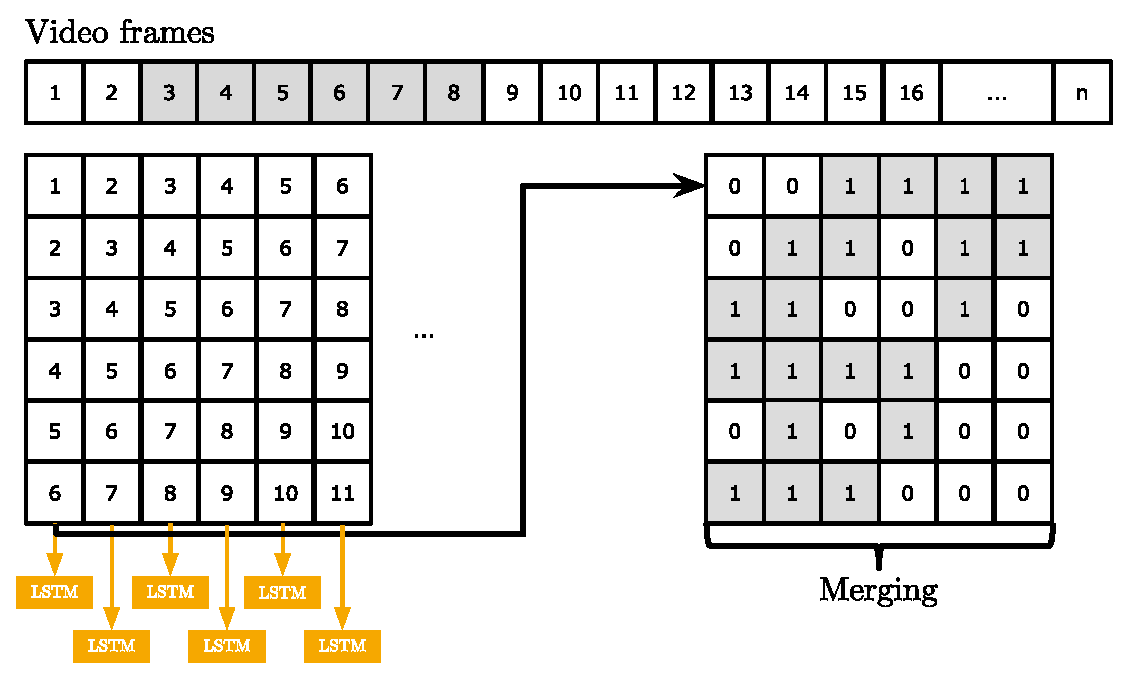
\includegraphics[scale=.7]{images/soft_cut_approach.eps}
	\caption{To classify soft cuts of arbitrary length, we repeatedly test fixed-size frame sequences. In this example we test sequences of size six. Afterwards the predictions given by the LSTM are merged, so that we have one prediction per frame.}
	\label{fig:soft_cut_approach}
\end{figure}
We have a video with \textit{n} frames.
The frames from three to eight represent a soft cut.
Now, for each frame, we generate a frame sequence of size six starting from that frame.
This is equivalent to moving a sliding window over the frames.
Those sequences are then classified by the LSTM.
The output of the LSTM is zero, if a frame does not belong to a soft cut, and one, otherwise.
In the end, we have up to six predictions per frame, which have to be merged, so that we have only one prediction per frame.
After merging, consecutive frames with a predicted value of 1 represent one soft cut.

In the following several strategies for combining multiple frame predictions into one prediction are presented.
An overview over all strategies can be found in Figure~\ref{fig:merging_strategies}.
\begin{figure}[!htb]
	\centering
	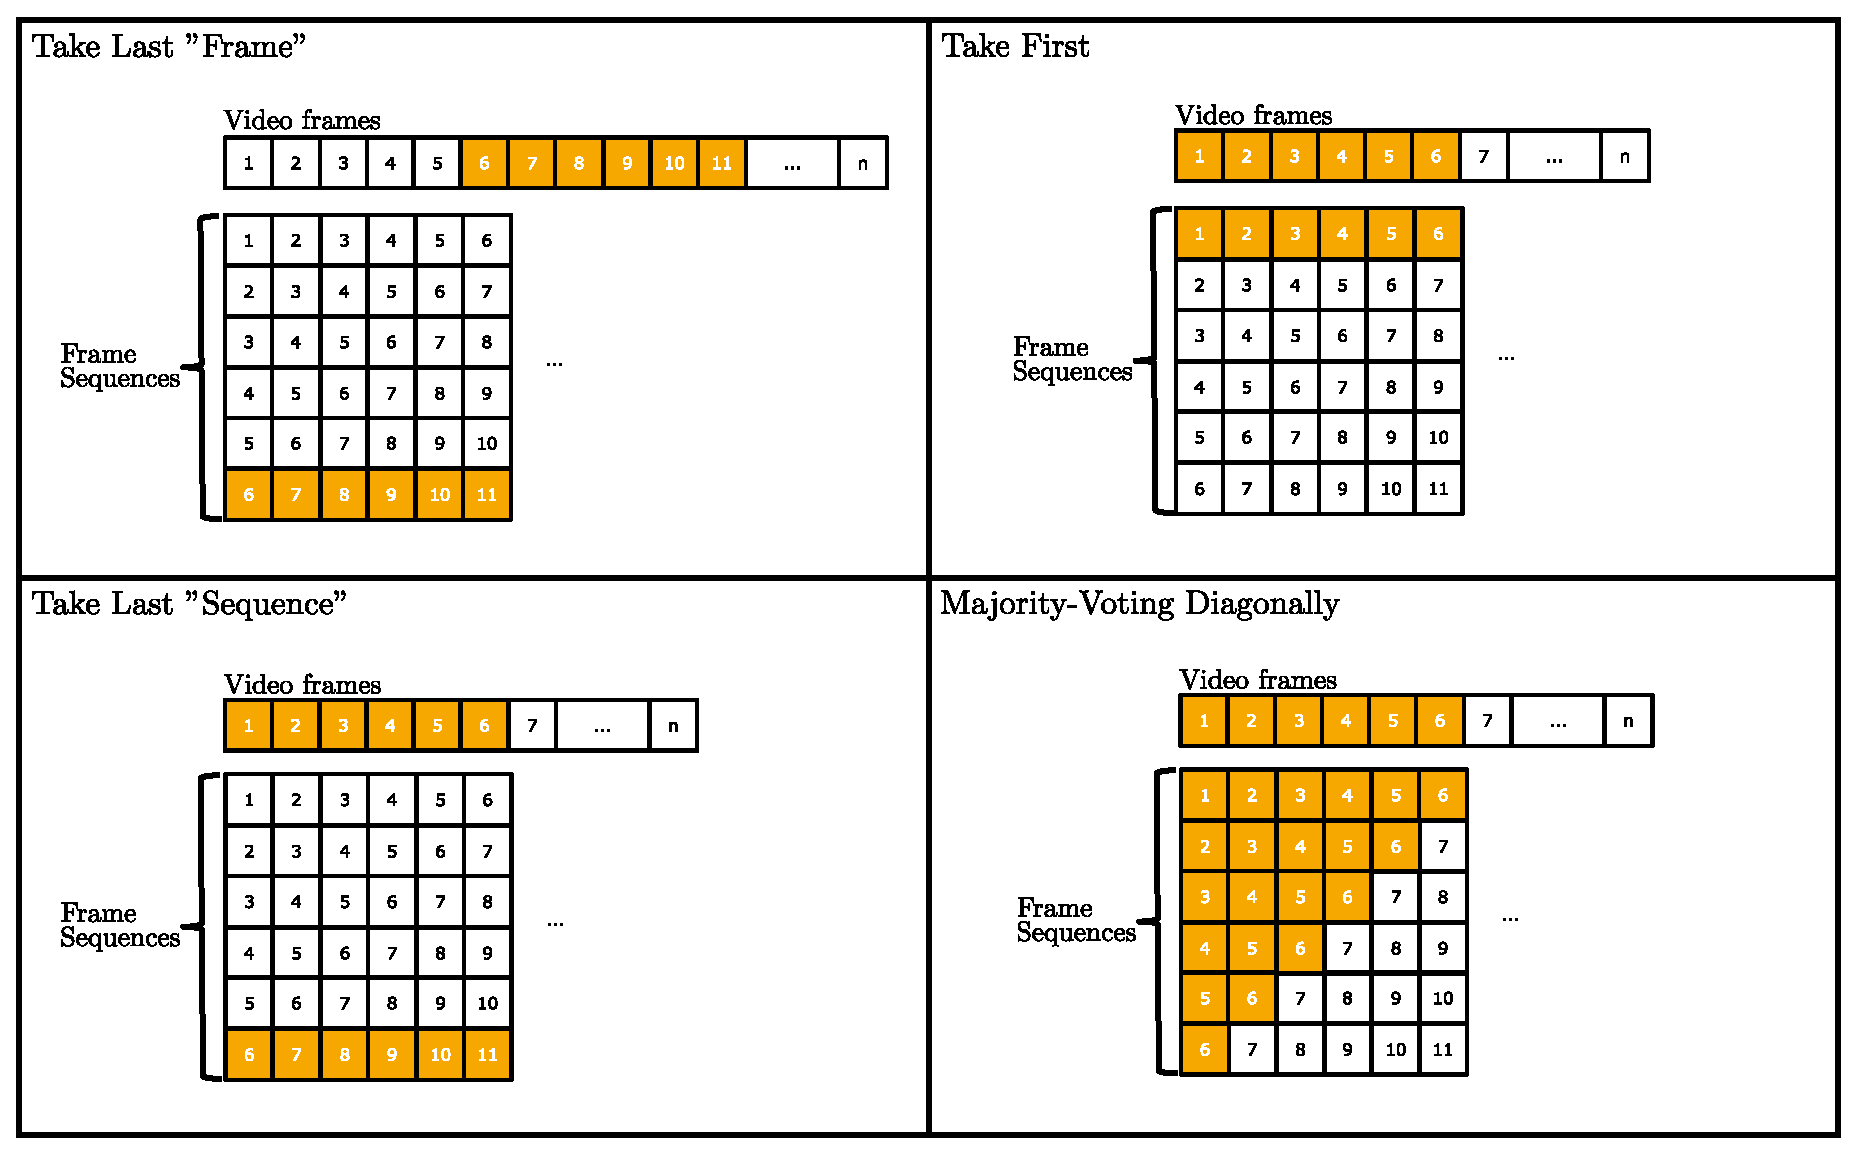
\includegraphics[scale=.5]{images/merging_strategies.eps}
	\caption{To merge the multiple predictions per frame into one, we implemented several strategies:
    \textit{Take Last 'Frame'} (top left): The prediction of the frame, where the frame is the last of a frame sequence, is taken.
    \textit{Take Last 'Sequence'} (bottom left): The last prediction of the frame sequence belonging to a frame is taken.
    \textit{Take First} (top right): The first prediction of the frame sequence is taken.
    \textit{Majority-Voting Diagonally} (bottom right): The majority voting among all predictions of the frame is taken.}
	\label{fig:merging_strategies}
\end{figure}
\paragraph{Take First}
A first simple strategy is to take the first prediction of each sequence as the prediction of that frame.
This is equivalent to having no prior knowledge about the frame, as the LSTM has not seen any previous frames and therefore could not remember anything.

\paragraph{Take Last 'Sequence'}
A second simple strategy is to take the last prediction of each sequence as the prediction for the frame that started the sequence.
Concretely, the last prediction is not a prediction for the frame under question, but the intuition behind this is that an LSTM becomes more and more certain after having seen multiple frames of the sequence.

\paragraph{Take Last 'Frame'}
In the \textit{Take Last 'Frame'} strategy, for every frame we take the frame sequence, in which that frame is the last one.
The intuition is similar to the previous case, but now we also use the prediction for the actual frame.

\paragraph{Majority-Voting Diagonally}
Each frame is predicted up to \textit{n} times.
In our example it is up to six times.
In the \textit{Majority-Voting Diagonally} all of those predictions are taken and the majority voting among those is taken as prediction for the frame.
Ties are resolved by placing more weight on the half of the predictions, where the frame appeared later in the sequence.

\subsubsection{Gap Filler}
After merging, we have one prediction per frame indicating whether the frame is part of a soft cut or not.
Then, a sequence of frames that are part of a soft cut represents a soft cut.
However, there could be misclassified frame predictions.
We implemented a \textit{Gap Filler} to find and correct some of those misclassified frame predictions.
The \textit{Gap Filler} is looking for sequences of frames that belong to a soft cut and are interrupted by some non cut frames.
If the number of interrupting frames is not too large, they are also classified as soft cut frames.
The idea behind the \textit{Gap Filler} is that two soft cuts do not occur close to each other.
So, if two soft cuts are only a few frames apart, they probably belong to the same soft cut.
In Figure~\ref{fig:gap_filler} an example of the \textit{Gap Filler} is shown.
There, a sequence of soft cut frames is interrupted by two non soft cut frames.
Those non soft cut frames are detected by the \textit{Gap Filler} and classified as soft cut frames.
\begin{figure}[!htb]
	\centering
	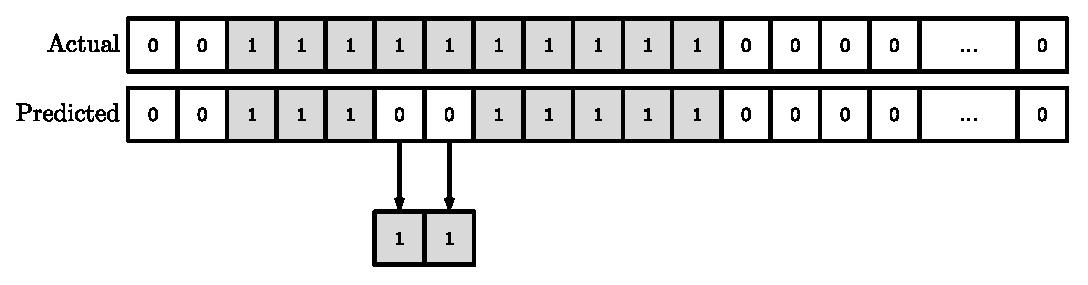
\includegraphics[scale=.7]{images/gap_filler.eps}
	\caption{Two soft cuts do not occur close to each other. Therefore the \textit{Gap Filler} finds misclassified frame predictions after the merging step and corrects non soft cut frame predictions, if they are interrupting a soft cut.}
	\label{fig:gap_filler}
\end{figure}

The gap filler presented so far is recall-oriented: It increases the recall of soft cuts, while trading precision at the same time.
By switching the roles of 0s and 1s, we can make the \textit{Gap Filler} also precision-oriented:
In this case, sequences of 1s, which are not long enough, are filled with 0s.

\subsubsection{Network Architectures}
To classify the frames as soft cut or non soft cut frames, we used an LSTM.
We tested many different architectures, and parameters settings.
In the following we present a selection of that with significant differences:

\paragraph{CNN + one LSTM}
For the CNN we used the architecture of the \textit{Caffenet}\footnote{\url{https://github.com/BVLC/caffe/tree/master/models/bvlc_reference_caffenet}}.
We also used the pre-trained weights of this net, so that we do not need to train our model from scratch.
We only fine-tuned the \textit{fc6} layer of the \textit{Caffenet} with a learning rate of 0.1.
The CNN is followed by one LSTM, whose weights were initialized with the \textit{Xavier} method, because this method performs better than other as mentioned in~\cite{glorot2010understanding}.
Besides, the general learning rate was set to 0.01 and gradient clipping was used.

\paragraph{CNN + two LSTMs}
The architecture of this net is basically the same as the previous.
There is only one difference: Instead of using just one LSTM, two LSTMs were used.
Also the general learning rate was set to 0.001 and no gradient clipping was used.
The architecture of the net can be found in Figure~\ref{fig:net_architecture}.
\begin{figure}[!htb]
	\centering
	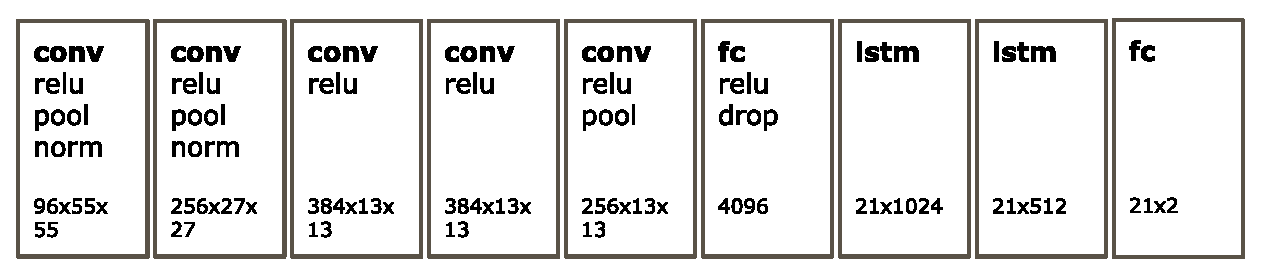
\includegraphics[scale=.5]{images/net_architecture.eps}
	\caption{Architecture of the LSTM consisting of a CNN and two LSTMs.}
	\label{fig:net_architecture}
\end{figure}

\paragraph{One convolutional layer + two LSTMs}
The last architecture that was tested uses only one convolutional layer before the two LSTMs.
The intuition behind it is as follows: for the CNN, it is hard to detect a soft cut frame, because it works only on one frame.
By looking at only one frame, it would be difficult to predict a soft cut, even for a human.
However, by looking at a sequence of frames, this becomes easier.
This is exactly, what the LSTM does, which is why we put more emphasis on this part and less emphasis on the CNN part.
The net was trained from scratch as no pre-trained net existed.
The weights of the LSTMs were again initialized using the \textit{Xavier} method.
The learning rate was 0.001 and gradient clipping was used during training.

